\documentclass[12pt]{article}
\usepackage[spanish]{babel}
\usepackage[utf8]{inputenc}
\usepackage[T1]{fontenc}
\usepackage{FiraSans}
\usepackage{amsmath}
\usepackage{graphicx}
\usepackage{float}
\usepackage{subfig}
\usepackage{array}
\renewcommand{\familydefault}{\sfdefault}
\renewcommand{\arraystretch}{1.05}

\begin{document}

\begin{titlepage}
\newcommand{\HRule}{\rule{\linewidth}{0.5mm}} 
\center


\includegraphics[scale=0.4]{images/logo-usm.png}\\
\vspace{0.6cm}
\textsc{\large INF480}\\[0.5cm] % Minor heading such as course title
\textsc{\Large Redes Complejas}\\[0.5cm] % Major heading such as course name

\HRule \\[0.4cm]
{ \huge \bfseries Tarea 2}\\[0.4cm] % Title of your document
\HRule \\[1.5cm]
 
\begin{minipage}{0.8\textwidth}
\begin{center} \large
Florencia Ramírez, ROL: 202073522-0\\
Sofía Riquelme, ROL: 202073615-4
\end{center}

\end{minipage}\\[2cm]

\vfill 

\end{titlepage}
\begin{enumerate}
    \item La matriz laplaciana del grafo es la siguiente:

    \[
    \begin{bmatrix}
        2 & -1 & -1 &  0 &  0 &  0 &  0 \\
        -1 &  2 & -1 &  0 &  0 &  0 &  0 \\
        -1 & -1 &  3 & -1 &  0 &  0 &  0 \\
        0 &  0 & -1 &  3 & -1 & -1 &  0 \\
        0 &  0 &  0 & -1 &  2 & -1 &  0 \\
        0 &  0 &  0 & -1 & -1 &  3 & -1 \\
        0 &  0 &  0 &  0 &  0 & -1 &  1
    \end{bmatrix}
    \]

    El valor de Fiedler para esta matriz es $0.34032095848177074$ y el vector propio asociado es el siguiente: 
    \[
    \begin{bmatrix}
         -0.46724728 \\
         -0.46724728 \\
         -0.30823323 \\
          0.11469308 \\
          0.27370712 \\
          0.33957289 \\
          0.5147547 
    \end{bmatrix}
    \]

    Luego, el gráfico de la red con sus comunidades es el siguiente:
    \begin{figure}[H]
        \begin{center}
            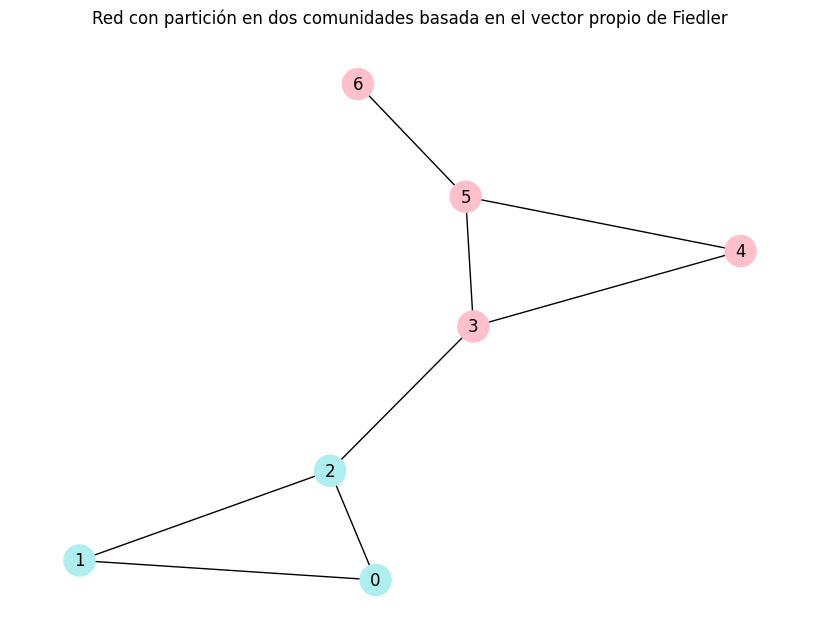
\includegraphics[scale=0.4]{images/grafico_red.png}
        \end{center}
        \caption{Gráfico de red}
        \label{fig:graph}
    \end{figure}

    \item 
    \begin{enumerate}
        \item Para que $P$ sea una distribución de probabilidad, debe ocurrir lo siguiente:
        $$\sum_{k=0}^{\infty}  P(k) = 1 $$
        Luego, dado que $P(k) = C \times \alpha ^k$, se tiene que 
        $$\sum_{k=0}^{\infty} C \alpha ^k= 1 $$
        Esto es una serie geométrica. La serie geométrica infinita $( \sum_{k=0}^{\infty} \alpha^k )$ converge a $( \frac{1}{1-\alpha} )$ siempre que $( |\alpha| < 1 )$. Por lo tanto,
        $$ \sum_{k=0}^{\infty} C \alpha ^k= C \left(\frac{1}{1-\alpha}\right) = 1 $$
        Despejando $C$:
        $$C = 1-\alpha$$

        \item La función generadora de un grafo, es $G_p(x) = \sum p_k x^k$. Como se vio en el ítem anterior, tenemos que $P(k) = C\alpha^k$ y $C = 1-\alpha$. Si sustituimos, se tiene que: 
        $$G(x) = \sum_{k=0}^{\infty}(1-\alpha)\alpha^k x^k$$ 
        $$G(x) = (1-\alpha)\sum_{k=0}^{\infty}(\alpha x)^k$$ 
        Utilizando la misma convergencia de series geométricas, se tiene que la expresión generadora para la distribución de grados es:
        $$G(x) = (1-\alpha)\left(\frac{1}{1-\alpha x}\right)$$

        \item no sé lol
    \end{enumerate}
    \newpage
    \item Al hacer las eliminaciones se obtuvieron los siguientes resultados:
    \begin{table}[H]
        \footnotesize
        \centering
        \begin{tabular}{|l|c|c|c|c|}
            \hline
            \textbf{Red} & \textbf{Nodos Iniciales} & \textbf{Aleatorio} & \textbf{Por Grado} & \textbf{Por Betweenness} \\
            \hline
            Piratas & $795$ & $33.33\%$ & $3.02\%$ & $3.14\%$ \\
            \hline
            Delfines & $62$ & $41.94\%$ & $24.19\%$ & $12.90\%$ \\
            \hline
            ER Piratas & $795$ & $24.40\%$ & $8.18\%$ & $5.16\%$ \\
            \hline
            ER Delfines & $62$ & $43.55\%$ & $30.65\%$ & $29.03\%$ \\
            \hline
        \end{tabular}
        \caption{Resumen de Eliminaciones en Diferentes Redes}
        \label{tabla:resumen_eliminaciones}
    \end{table}

    \item 
    
    \item 
    
    \item
    \begin{enumerate}
        \item El gráfico de la red es el siguiente:
        \begin{figure}[H]
            \centering
            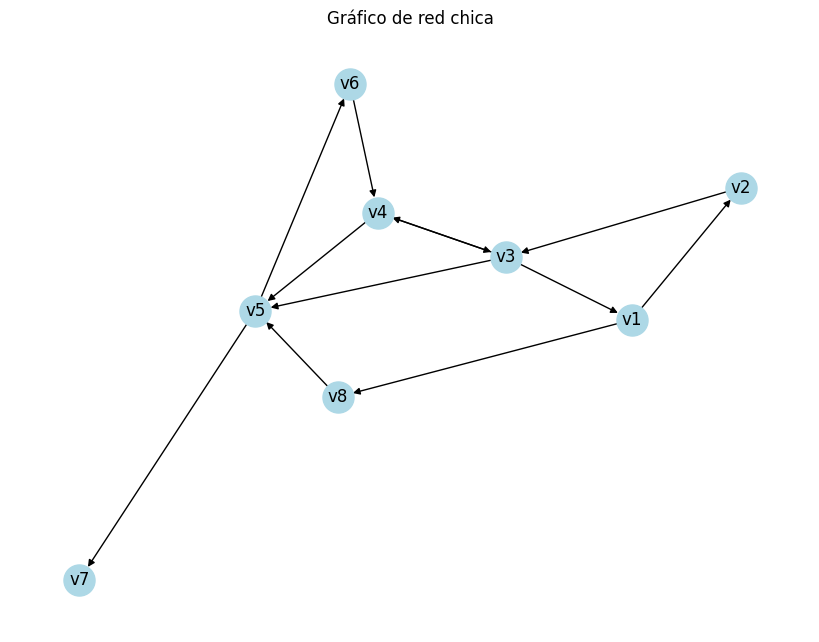
\includegraphics[scale=0.5]{images/grafico_red_chica.png}
            \caption{Gráfico de red chica}
            \label{fig:graph_red_chica}
        \end{figure}

        Los valores del grado de entrada, betweenness y PageRank de cada nodo son:
        
        \begin{table}[H]
            \centering
            \begin{tabular}{|c|c|c|c|}
            \hline
            Nodo & Grado de entrada & Betweenness & PageRank \\ \hline
            v1 & $1$ & $0,238095$ & $0,077725$ \\ \hline
            v2 & $1$ & $0,047619$ & $0,064579$ \\ \hline
            v3 & $2$ & $0,428571$ & $0,162980$ \\ \hline
            v4 & $2$ & $0,309524$ & $0,180098$ \\ \hline
            v5 & $3$ & $0,357143$ & $0,209159$ \\ \hline
            v6 & $1$ & $0,214286$ & $0,120440$ \\ \hline
            v7 & $1$ & $0,000000$ & $0,120440$ \\ \hline
            v8 & $1$ & $0,071429$ & $0,064579$ \\ \hline
            \end{tabular}
            \caption{Valores de grado de entrada, betweenness y PageRank}
            \label{tab:values_red_chica}
        \end{table}

        \item El ranking de los nodos según su grado de entrada sería:
        \begin{enumerate}
            \item v5
            \item v3 y v4
            \item v1, v2, v6, v7 y v8
        \end{enumerate}

        Luego, el ranking de los nodos según su betweenness sería:
        \begin{enumerate}
            \item v3
            \item v4
            \item v5
            \item v1
            \item v6
            \item v2
            \item v8
            \item v7
        \end{enumerate}

        Finalmente, el ranking de los nodos según su valor de PageRank sería:
        \begin{enumerate}
            \item v5
            \item v4
            \item v3
            \item v6 y v7
            \item v1
            \item v2 y v8
        \end{enumerate}

        \item Se puede observar una relación entre grado de entrada, betweenness y valor de PageRank, los nodos con mayor grado de entrada también tienden a tener mayor valores de betweenness y PageRank, que se puede observar en los nodos v3, v4 y v5.
        
        más chamullo :>
    \end{enumerate}
    
\end{enumerate}


\end{document}